\documentclass[12pt]{article}

\usepackage{amsmath, amssymb}
\usepackage[margin=1in]{geometry}
\usepackage{helvet}
\renewcommand{\familydefault}{\sfdefault}
\def\newrule#1#2#3{\begin{center}
    {#1} \\
    \line(1,0){300} {}{}{}{}{}{}{} [{#3}]\\
    {#2}
\end{center}}

\begin{document}
\def\assignment{Homework 04}

\pagenumbering{gobble}
\noindent{\large COSC 4200 \hfill Name: \underline{Jacob Tuttle} \\ Computability and Complexity}
\begin{center}
    {\Large \assignment} \\ \textbf{\today}
\end{center}

\begin{enumerate}
    \item Suppose $ADD$ is regular. Let $p$ be the pumping constant for $ADD$. Let $w = a^pb^pc^{2p}$. Then $w$ can be broken up into substrings $xyz$ where $|xy| \leq p$ and $0 \leq |y|$ such that $xy^iz$ exists for all $i$. \\

    Then we know that $x = a^k, y = a^j,$ and $z=a^{p-k-j}b^pc^{2p}$ where $k \geq 0, j > 0$. \\

    Let $i = 2$. Then:
    \begin{align*}
        xy^2z &= a^ka^{2j}a^{p-k-j}b^pc^{2p} \\
        &= a^{p+j}b^pc^{2p} \in ADD
    \end{align*}

    But since $j > 0, 2p+j \neq 2p$ Thus, there are more as and bs than $ADD$ is able to accept. Since this is a contradiction to our assumption that $ADD$ is regular, we know that it must be nonregular.

    \item Suppose $POWERS$ is regular. Let $p$ be the pumping constant for $POWERS$. Let $w = 0^{2^p}$. Then $w$ can be broken up into substrings $xyz$ where $|xy| \leq p$ and $0 \leq |y|$ such that $xy^iz$ exists for all $i$. \\

    Then we know that $x = 0^k, y = 0^j,$ and $z=0^{2^p - k - j}$ where $k \geq 0, j > 0$. \\

    Let $i = 2$. Then:
    \begin{align*}
        xy^2z &= 0^k0^{2j}0^{2^p - k - j} \\
        &= 0^{2^p + j} \in POWERS
    \end{align*}

    But since $j > 0, 2^p + j \neq 2^p$ Thus, there are more as and bs than $POWERS$ is able to accept. Since this is a contradiction to our assumption that $POWERS$ is regular, we know that it must be nonregular.

    \item \begin{enumerate}
        \item $A \to 0A0 | 0A1 | 1A0 | 1A1 | 1$

        \item $A \to 0A0 | 1A1 | 1 | 0 | \epsilon$

        \item $A \to 0B0 | 0B1 | 1B0 | 1B1 | B$ \\ $B \to A | 01 | 10$

        \item $A \to aFbC | aS | \epsilon$ \\ $F \to aFb | \epsilon$ \\ $S \to bSc | \epsilon$ \\ $C \to cC | \epsilon$

        \item $A \to BbbaB$ \\ $B \to aB | bB | \epsilon$

        \item $A \to AaA | AbaA | AbbB | B | \epsilon$ \\ $B \to bB | \epsilon$

        \item $A \to aab | aaAB | a$ \\ $B \to b | \epsilon$

        \item $S \to aSd | aDc | bAd | bMc$ \\ $D \to aDc | bMc | \epsilon$ \\ $A \to bMc | bAd | \epsilon$ \\ $M \to bMc | \epsilon$
    \end{enumerate}

    \item \begin{enumerate}
        \item This PDA works by pushing two as to the stack for every one it reads. Then, when it comes time to read the bs, it pops off one a for each b. If there are twice as many bs as as that were read in, it will end up in an accepting state.
        \begin{center}
        \begin{tikzpicture}[scale=0.2]
        \tikzstyle{every node}+=[inner sep=0pt]
        \draw [black] (11,-9.8) circle (3);
        \draw [black] (27.2,-9.8) circle (3);
        \draw [black] (44.5,-9.8) circle (3);
        \draw [black] (64,-24.6) circle (3);
        \draw [black] (64,-24.6) circle (2.4);
        \draw [black] (64,-9.8) circle (3);
        \draw [black] (4.2,-9.8) -- (8,-9.8);
        \fill [black] (8,-9.8) -- (7.2,-9.3) -- (7.2,-10.3);
        \draw [black] (14,-9.8) -- (24.2,-9.8);
        \fill [black] (24.2,-9.8) -- (23.4,-9.3) -- (23.4,-10.3);
        \draw (19.1,-10.3) node [below] {$\epsilon,\mbox{ }\epsilon\mbox{ }\to\mbox{ }\$$};
        \draw [black] (30.06,-8.902) arc (103.87314:76.12686:24.146);
        \fill [black] (41.64,-8.9) -- (40.98,-8.22) -- (40.74,-9.2);
        \draw (35.85,-7.7) node [above] {$a,\mbox{ }\epsilon\mbox{ }\to\mbox{ }a$};
        \draw [black] (64,-12.8) -- (64,-21.6);
        \fill [black] (64,-21.6) -- (64.5,-20.8) -- (63.5,-20.8);
        \draw (63.5,-17.2) node [left] {$\epsilon,\mbox{ }\$\mbox{ }\to\mbox{ }\epsilon$};
        \draw [black] (47.5,-9.8) -- (61,-9.8);
        \fill [black] (61,-9.8) -- (60.2,-9.3) -- (60.2,-10.3);
        \draw (54.25,-10.3) node [below] {$b,\mbox{ }a\mbox{ }\to\mbox{ }\epsilon$};
        \draw [black] (66.68,-8.477) arc (144:-144:2.25);
        \draw (71.25,-9.8) node [right] {$b,\mbox{ }a\mbox{ }\to\mbox{ }\epsilon$};
        \fill [black] (66.68,-11.12) -- (67.03,-12) -- (67.62,-11.19);
        \draw [black] (41.832,-11.162) arc (-68.27418:-111.72582:16.16);
        \fill [black] (29.87,-11.16) -- (30.43,-11.92) -- (30.8,-10.99);
        \draw (35.85,-12.81) node [below] {$\epsilon,\mbox{ }\epsilon\mbox{ }\to\mbox{ }a$};
        \end{tikzpicture}
        \end{center}

        \item This PDA will read in the first half until you have pushed a 1 and then pop off a 1 indicating that there is a 11 in the middle of the input string, and then begins popping elements off of the stack.
        \begin{center}
        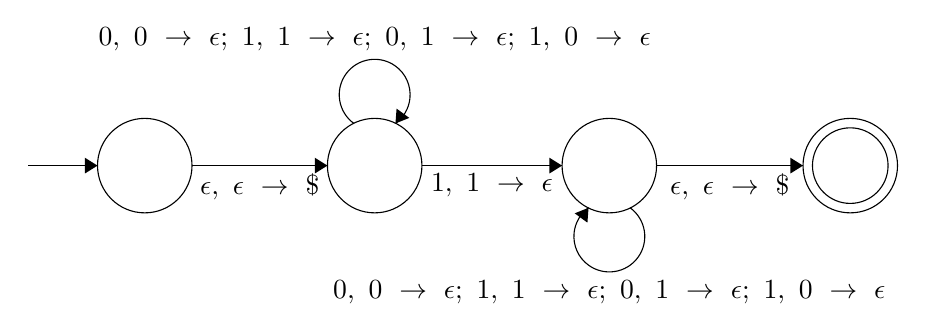
\begin{tikzpicture}[scale=0.2]
        \tikzstyle{every node}+=[inner sep=0pt]
        \draw [black] (9.6,-13.4) circle (3);
        \draw [black] (24.2,-13.4) circle (3);
        \draw [black] (39.1,-13.4) circle (3);
        \draw [black] (54.4,-13.4) circle (3);
        \draw [black] (54.4,-13.4) circle (2.4);
        \draw [black] (2.2,-13.4) -- (6.6,-13.4);
        \fill [black] (6.6,-13.4) -- (5.8,-12.9) -- (5.8,-13.9);
        \draw [black] (42.1,-13.4) -- (51.4,-13.4);
        \fill [black] (51.4,-13.4) -- (50.6,-12.9) -- (50.6,-13.9);
        \draw (46.75,-13.9) node [below] {$\epsilon,\mbox{ }\epsilon\mbox{ }\to\mbox{ }\$$};
        \draw [black] (27.2,-13.4) -- (36.1,-13.4);
        \fill [black] (36.1,-13.4) -- (35.3,-12.9) -- (35.3,-13.9);
        \draw (31.65,-13.9) node [below] {$1,\mbox{ }1\mbox{ }\to\mbox{ }\epsilon$};
        \draw [black] (40.423,-16.08) arc (54:-234:2.25);
        \draw (39.1,-20.65) node [below] {$0,\mbox{ }0\mbox{ }\to\mbox{ }\epsilon;\mbox{ }1,\mbox{ }1\mbox{ }\to\mbox{ }\epsilon;\mbox{ }0,\mbox{ }1\mbox{ }\to\mbox{ }\epsilon;\mbox{ }1,\mbox{ }0\mbox{ }\to\mbox{ }\epsilon$};
        \fill [black] (37.78,-16.08) -- (36.9,-16.43) -- (37.71,-17.02);
        \draw [black] (12.6,-13.4) -- (21.2,-13.4);
        \fill [black] (21.2,-13.4) -- (20.4,-12.9) -- (20.4,-13.9);
        \draw (16.9,-13.9) node [below] {$\epsilon,\mbox{ }\epsilon\mbox{ }\to\mbox{ }\$$};
        \draw [black] (22.877,-10.72) arc (234:-54:2.25);
        \draw (24.2,-6.15) node [above] {$0,\mbox{ }0\mbox{ }\to\mbox{ }\epsilon;\mbox{ }1,\mbox{ }1\mbox{ }\to\mbox{ }\epsilon;\mbox{ }0,\mbox{ }1\mbox{ }\to\mbox{ }\epsilon;\mbox{ }1,\mbox{ }0\mbox{ }\to\mbox{ }\epsilon$};
        \fill [black] (25.52,-10.72) -- (26.4,-10.37) -- (25.59,-9.78);
        \end{tikzpicture}
        \end{center}

        \item Read 0s and fill the stack, then pop them off each time we read a 1. If we read a 1 and pop a \$ off the stack, that means that there are more 1s than 0s, so we move to an accepting state and read through the rest of the input string.
        \begin{center}
        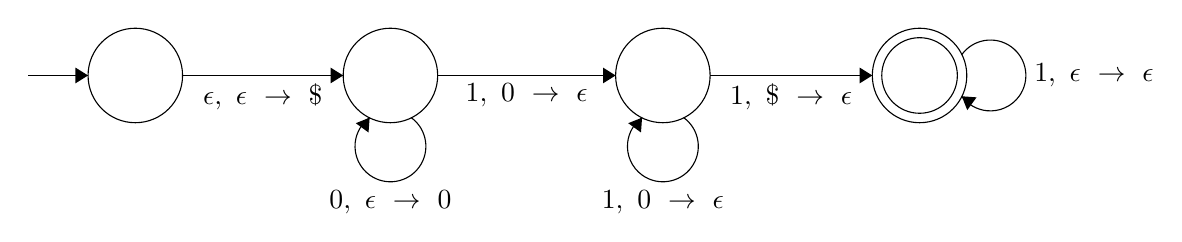
\begin{tikzpicture}[scale=0.2]
        \tikzstyle{every node}+=[inner sep=0pt]
        \draw [black] (11,-9.8) circle (3);
        \draw [black] (27.2,-9.8) circle (3);
        \draw [black] (44.5,-9.8) circle (3);
        \draw [black] (60.8,-9.8) circle (3);
        \draw [black] (60.8,-9.8) circle (2.4);
        \draw [black] (63.48,-8.477) arc (144:-144:2.25);
        \draw (68.05,-9.8) node [right] {$1,\mbox{ }\epsilon\mbox{ }\to\mbox{ }\epsilon$};
        \fill [black] (63.48,-11.12) -- (63.83,-12) -- (64.42,-11.19);
        \draw [black] (4.2,-9.8) -- (8,-9.8);
        \fill [black] (8,-9.8) -- (7.2,-9.3) -- (7.2,-10.3);
        \draw [black] (14,-9.8) -- (24.2,-9.8);
        \fill [black] (24.2,-9.8) -- (23.4,-9.3) -- (23.4,-10.3);
        \draw (19.1,-10.3) node [below] {$\epsilon,\mbox{ }\epsilon\mbox{ }\to\mbox{ }\$$};
        \draw [black] (30.2,-9.8) -- (41.5,-9.8);
        \fill [black] (41.5,-9.8) -- (40.7,-9.3) -- (40.7,-10.3);
        \draw (35.85,-10.3) node [below] {$1,\mbox{ }0\mbox{ }\to\mbox{ }\epsilon$};
        \draw [black] (47.5,-9.8) -- (57.8,-9.8);
        \fill [black] (57.8,-9.8) -- (57,-9.3) -- (57,-10.3);
        \draw (52.65,-10.3) node [below] {$1,\mbox{ }\$\mbox{ }\to\mbox{ }\epsilon$};
        \draw [black] (45.823,-12.48) arc (54:-234:2.25);
        \draw (44.5,-17.05) node [below] {$1,\mbox{ }0\mbox{ }\to\mbox{ }\epsilon$};
        \fill [black] (43.18,-12.48) -- (42.3,-12.83) -- (43.11,-13.42);
        \draw [black] (28.523,-12.48) arc (54:-234:2.25);
        \draw (27.2,-17.05) node [below] {$0,\mbox{ }\epsilon\mbox{ }\to\mbox{ }0$};
        \fill [black] (25.88,-12.48) -- (25,-12.83) -- (25.81,-13.42);
        \end{tikzpicture}
        \end{center}


        \item This PDA will use a non-deterministic approach to split the input into one of two branches that will accept if $i = k$ on the left or $j = l$ on the right.
        \begin{center}
        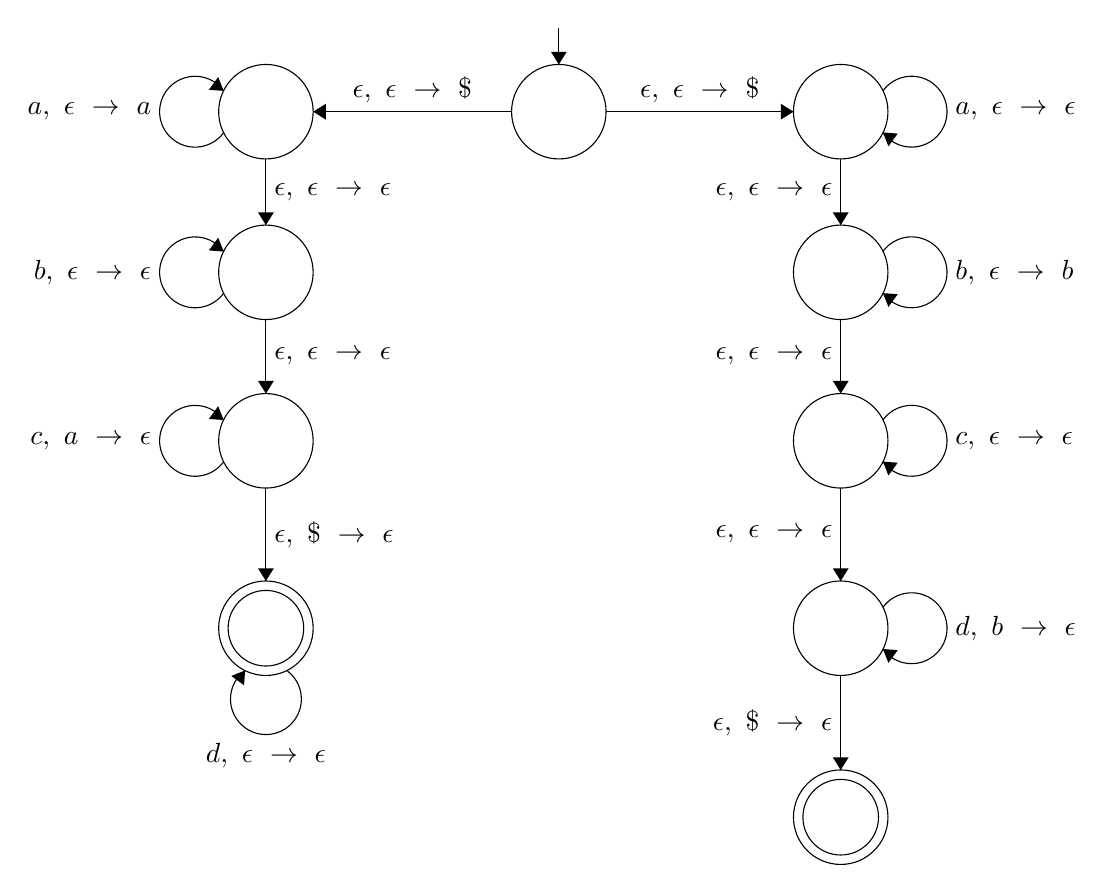
\begin{tikzpicture}[scale=0.2]
        \tikzstyle{every node}+=[inner sep=0pt]
        \draw [black] (39.6,-7) circle (3);
        \draw [black] (21,-7) circle (3);
        \draw [black] (21,-17.2) circle (3);
        \draw [black] (21,-27.9) circle (3);
        \draw [black] (21,-39.8) circle (3);
        \draw [black] (21,-39.8) circle (2.4);
        \draw [black] (57.5,-7) circle (3);
        \draw [black] (57.5,-17.2) circle (3);
        \draw [black] (57.5,-39.8) circle (3);
        \draw [black] (57.5,-27.9) circle (3);
        \draw [black] (57.5,-51.8) circle (3);
        \draw [black] (57.5,-51.8) circle (2.4);
        \draw [black] (39.6,-1.7) -- (39.6,-4);
        \fill [black] (39.6,-4) -- (40.1,-3.2) -- (39.1,-3.2);
        \draw [black] (36.6,-7) -- (24,-7);
        \fill [black] (24,-7) -- (24.8,-7.5) -- (24.8,-6.5);
        \draw (30.3,-6.5) node [above] {$\epsilon,\mbox{ }\epsilon\mbox{ }\to\mbox{ }\$$};
        \draw [black] (42.6,-7) -- (54.5,-7);
        \fill [black] (54.5,-7) -- (53.7,-6.5) -- (53.7,-7.5);
        \draw (48.55,-6.5) node [above] {$\epsilon,\mbox{ }\epsilon\mbox{ }\to\mbox{ }\$$};
        \draw [black] (21,-10) -- (21,-14.2);
        \fill [black] (21,-14.2) -- (21.5,-13.4) -- (20.5,-13.4);
        \draw (21.5,-12.1) node [right] {$\epsilon,\mbox{ }\epsilon\mbox{ }\to\mbox{ }\epsilon$};
        \draw [black] (57.5,-10) -- (57.5,-14.2);
        \fill [black] (57.5,-14.2) -- (58,-13.4) -- (57,-13.4);
        \draw (57,-12.1) node [left] {$\epsilon,\mbox{ }\epsilon\mbox{ }\to\mbox{ }\epsilon$};
        \draw [black] (57.5,-20.2) -- (57.5,-24.9);
        \fill [black] (57.5,-24.9) -- (58,-24.1) -- (57,-24.1);
        \draw (57,-22.55) node [left] {$\epsilon,\mbox{ }\epsilon\mbox{ }\to\mbox{ }\epsilon$};
        \draw [black] (57.5,-30.9) -- (57.5,-36.8);
        \fill [black] (57.5,-36.8) -- (58,-36) -- (57,-36);
        \draw (57,-33.85) node [left] {$\epsilon,\mbox{ }\epsilon\mbox{ }\to\mbox{ }\epsilon$};
        \draw [black] (57.5,-42.8) -- (57.5,-48.8);
        \fill [black] (57.5,-48.8) -- (58,-48) -- (57,-48);
        \draw (57,-45.8) node [left] {$\epsilon,\mbox{ }\$\mbox{ }\to\mbox{ }\epsilon$};
        \draw [black] (21,-20.2) -- (21,-24.9);
        \fill [black] (21,-24.9) -- (21.5,-24.1) -- (20.5,-24.1);
        \draw (21.5,-22.55) node [right] {$\epsilon,\mbox{ }\epsilon\mbox{ }\to\mbox{ }\epsilon$};
        \draw [black] (21,-30.9) -- (21,-36.8);
        \fill [black] (21,-36.8) -- (21.5,-36) -- (20.5,-36);
        \draw (21.5,-33.85) node [right] {$\epsilon,\mbox{ }\$\mbox{ }\to\mbox{ }\epsilon$};
        \draw [black] (18.32,-8.323) arc (-36:-324:2.25);
        \draw (13.75,-7) node [left] {$a,\mbox{ }\epsilon\mbox{ }\to\mbox{ }a$};
        \fill [black] (18.32,-5.68) -- (17.97,-4.8) -- (17.38,-5.61);
        \draw [black] (18.32,-18.523) arc (-36:-324:2.25);
        \draw (13.75,-17.2) node [left] {$b,\mbox{ }\epsilon\mbox{ }\to\mbox{ }\epsilon$};
        \fill [black] (18.32,-15.88) -- (17.97,-15) -- (17.38,-15.81);
        \draw [black] (18.32,-29.223) arc (324:36:2.25);
        \draw (13.75,-27.9) node [left] {$c,\mbox{ }a\mbox{ }\to\mbox{ }\epsilon$};
        \fill [black] (18.32,-26.58) -- (17.97,-25.7) -- (17.38,-26.51);
        \draw [black] (60.18,-5.677) arc (144:-144:2.25);
        \draw (64.75,-7) node [right] {$a,\mbox{ }\epsilon\mbox{ }\to\mbox{ }\epsilon$};
        \fill [black] (60.18,-8.32) -- (60.53,-9.2) -- (61.12,-8.39);
        \draw [black] (60.18,-15.877) arc (144:-144:2.25);
        \draw (64.75,-17.2) node [right] {$b,\mbox{ }\epsilon\mbox{ }\to\mbox{ }b$};
        \fill [black] (60.18,-18.52) -- (60.53,-19.4) -- (61.12,-18.59);
        \draw [black] (60.18,-26.577) arc (144:-144:2.25);
        \draw (64.75,-27.9) node [right] {$c,\mbox{ }\epsilon\mbox{ }\to\mbox{ }\epsilon$};
        \fill [black] (60.18,-29.22) -- (60.53,-30.1) -- (61.12,-29.29);
        \draw [black] (60.18,-38.477) arc (144:-144:2.25);
        \draw (64.75,-39.8) node [right] {$d,\mbox{ }b\mbox{ }\to\mbox{ }\epsilon$};
        \fill [black] (60.18,-41.12) -- (60.53,-42) -- (61.12,-41.19);
        \draw [black] (22.323,-42.48) arc (54:-234:2.25);
        \draw (21,-47.05) node [below] {$d,\mbox{ }\epsilon\mbox{ }\to\mbox{ }\epsilon$};
        \fill [black] (19.68,-42.48) -- (18.8,-42.83) -- (19.61,-43.42);
        \end{tikzpicture}
        \end{center}
    \end{enumerate}

    \item To prove that context free languages are closed under union, concatenation, and star, we will construct a set of rules such that the grammars will incorporate those properties. Let us have two context free languages $S_1$ and $S_2$. To union the two langauges, construct a new language $S_1 \cup S_2 \to S_1 | S_2$. To concatenate the two languages, construct a new language $S_1 \cdot S_2 \to S_1S_2$. To star closure a language, construct a new language for $S_1^* \to S_1S_1^* | \epsilon$.
\end{enumerate}
\end{document}
